\documentclass[12pt]{article}
\usepackage[a4paper, left=3.17cm, right=3.17cm, top=2.54cm, bottom=2.54cm]{geometry}
\usepackage{eurosym}
\usepackage{listings}
\lstset{framexleftmargin=5mm, frame=shadowbox, rulesepcolor=\color{blue}}
\lstdefinestyle{bash}{
language        =   bash,
breaklines      =   true
}
\usepackage[T1]{fontenc}
\usepackage{mathptmx}
\usepackage{amsmath}
\usepackage{booktabs}
\usepackage{amsfonts}
\usepackage{indentfirst}
\usepackage{chemformula}
\usepackage{graphicx}
\graphicspath{{figure/}}
\usepackage{float}
\usepackage[hypcap=true,labelsep=period,font=small]{caption}
\usepackage[hypcap=true]{subcaption}
\usepackage{biblatex}
\usepackage[final]{hyperref}
\hypersetup{
	colorlinks=true,       % false: boxed links; true: colored links
	linkcolor=black,        % color of internal links
	citecolor=black,        % color of links to bibliography
	filecolor=black,     % color of file links
	urlcolor=black         
}

\setlength{\parskip}{0.5em}
\title{Red Blue Computation Program Report}
\author{\textup{Zicong Wu}}
\date{\teday}
\begin{document}
    \begin{titlepage}
    \newcommand{\HRule}{\rule{\linewidth}{0.5mm}}
    \includegraphics[width=8cm]{title/logo.png}
    \center 
    \quad\\[1.5cm]
    \textsl{\Large The University of Sydney}\\[0.5cm] 
    \textsl{\large School of Electrical and Information Engineering}\\[0.5cm] 
    \makeatletter
    \HRule \\[0.4cm]
    { \huge \bfseries \@title}\\[0.4cm] 
    \HRule \\[1.5cm]
    \begin{minipage}{0.4\textwidth}
    \begin{flushleft} \large
    \emph{Student Name:}\\
    \@author 
    \end{flushleft}
    \end{minipage}
    ~
    \begin{minipage}{0.4\textwidth}
    \begin{flushright} \large
    \emph{SID:} \\
    \textup{500295324}
    \end{flushright}
    \end{minipage}\\[3cm]
    \makeatother
    {\large An Assignment submitted for the UoS:}\\[0.5cm]
    {\large \emph{COMP5426 Parallel and Distributed Computing}}\\[0.5cm]
    {\large \today}\\[2cm] 
    \vfill 
\end{titlepage}
    \tableofcontents
    \newpage

\section{Problem definition and requirements}
The Red/Blue computation is a simulation of an interaction between different movement of cells in a board. 
At the beginning the program need to ask user for 4 user define parameters: n, t, c and M, then the board was separated into n * n cells, every cell will be randomly colored into red and blue, with roughly 1/3 blue cells, 1/3 red cells and the rest are white. The board also be separated into $t \times t$ tiles, which mean every tile will contain $n/t \times n/t$ cells.
Each interaction was composed by two steps: first step, every red cell moves to their right if the cell on the right side is white. The second step is similar except the blue need to move down if the cell below is white. If the movement reach the edge of the board, they will be wraparound to the opposite side of the board.
The game will be terminated in two ways: one is that in any tile the number of red or blue cells is greater than $c\%$ of the size of the tile. Another is that the number of interactions happened to the board is equal to M. the program needs to detail about the terminal conduction.


\section{Parallel algorithm design}
The parallel algorithm design is based on Pthread library, the program can be separated into parameters input, grid initialization, operation and self-checking, \autoref{fig:flowchart}. To maintain the reusability of code between parallel and sequential computing, the sequential procedure and be treated as a special parallel procedure with only one thread. 
\begin{figure}[ht]
    \centering
    \subcaptionbox{Main\label{fig:main}}
    [0.48\textwidth]{\includegraphics[width=0.9\linewidth]{main.pdf}}
    \subcaptionbox{Work load function\label{fig:work}}
    [0.48\textwidth]{\includegraphics[width=0.9\linewidth]{workload.pdf}}
    \caption{The flow chart of essential code.}
    \label{fig:flowchart}
\end{figure}
\subsection{Parameters input}
The program will ask 5 user-defined parameters in \autoref{fig:main}, include the number of rows or columns in one dimension, the number of tiles in one dimension, the threshold in percentage, the maximum interaction be simulated and the number of thread created, it will check if the parameters are legal or not and calculate relative variables.
\subsection{Grid initialization}
After scan parameters from standard input output, a series of memory will be allocated by “malloc” function, which include a grid and memory store which tiles meet the terminal condition with which color, it will be the shared memory of different threads.
\subsection{Operation}
In the cell movement, one thread will control rows of grid when moving red cells, and will change to control columns to move blue, which will avoid threads modified a shared memory since the red cell only move to right if possible, and blue cells only move down, the interaction only happened internally instead of mutually which also avoided negotiation between bordering threads. The decomposing of threads can be illustrated by \autoref{fig:decompose}, in which the green rectangle represents the control area or one thread. As an example, in the red movement period, the thread control the fifth and sixth rows (horizontal green rectangle in \autoref{fig:decompose}), and move the red cell, in the period of moving blue cells, the thread change its control area to the fifth and sixth columns (vertical rectangle in \autoref{fig:decompose}) and conduct the movement. Since the movement of red and blue cell need to be synchronized, a mechanism called barrier was introduced to block the referencing threads until all the threads was blocked, which will guarantee the synchronization between threads. In this scenario, the barrier was inserted between red movement and blue movement (purple line between ``move red'' and ``move blue'' in \autoref{fig:work}).
\begin{figure}[ht]
    \centering
    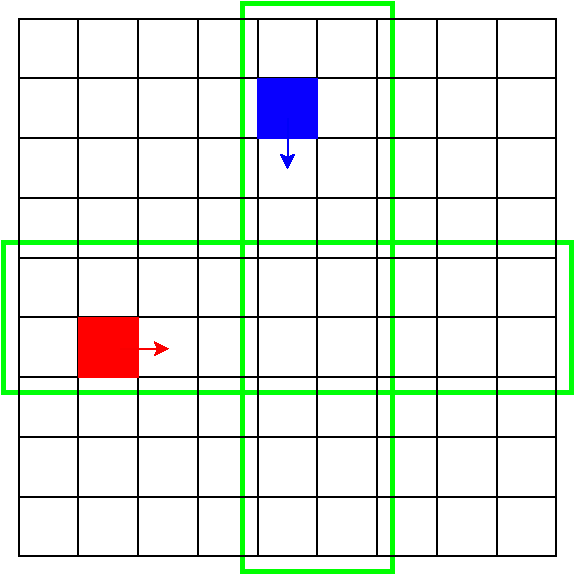
\includegraphics[width = 0.48 \textwidth]{move.pdf}
    \caption{Illustration of decomposing.}
    \label{fig:decompose}
\end{figure}

In the tile inspection, the tiles of the grid can be considered as a one dimension array, and will be equally assigned to threads, every thread will store the terminated tile address and terminated color in a local memory, later they will write to the shared memory in protection of ``Read Write Lock'' which was illustrated by the double line in \autoref{fig:work}, the red one is writing lock and green one is unlocking. The threads will first inspect tiles assigned to them and check the number of terminated tile in the shared memory to decide whether to stop the interaction. A barrier was inserted before checking the global terminated number and after the writing of the global terminated number, illustrated by the purple line in \autoref{fig:work}.

\section{Implementation and test}
The program stared with asking five user-defined parameters, input number as testing:
\begin{lstlisting}[style = bash]
Number of rows(n) in the board n:
9
Number of taills(t) in a dimension t:
3
Threshold(0<=c%<=100):
100
Nomber of threads(1<=thr<=9):
4
Maximum interactions:
50
\end{lstlisting}
The movement of cells and inspection of tiles is current, the initial and final grid was printed in standard I/O. 
\begin{table}[ht]
    \centering
    \caption{Test environment.}
    \label{tab:environment}
    \begin{tabular}{@{}cc@{}}
    \toprule
    {\color[HTML]{000000} Environment}      & {\color[HTML]{000000} value}                           \\ \midrule
    {\color[HTML]{000000} Operating system} & {\color[HTML]{000000} macOS Catalina V10.15.7}         \\
    {\color[HTML]{000000} CPU}              & {\color[HTML]{000000} Dual-Core Intel Core i5 @2.5GHz} \\
    {\color[HTML]{000000} RAM}              & {\color[HTML]{000000} 8G-DDR3-1600MHz}                 \\
    {\color[HTML]{000000} Compiler}         & {\color[HTML]{000000} Apple clang V11.0.3}             \\
    Shell                                   & zsh V5.7.1                                             \\ \bottomrule
    \end{tabular}
    \end{table}
Different set of the number of thread was tested in condition of parameters above and in environment of \autoref{tab:environment}, and the result is listed in \autoref{tab:test}, note that the result is the time duration of first time running and the second time running of the program.
\begin{table}[ht]
    \centering
    \caption{Test with different number of threads.}
    \label{tab:test}
    \begin{tabular}{@{}cccc@{}}
        \toprule
        {\color[HTML]{000000} Number of threads} & {\color[HTML]{000000} first times/s} & second times/s & Normalized \\ \midrule
        {\color[HTML]{000000} 1}                 & {\color[HTML]{000000} 0.553}         & 0.2            & 1.00       \\
        {\color[HTML]{000000} 2}                 & {\color[HTML]{000000} 0.357}         & 0.11           & 0.20       \\
        {\color[HTML]{000000} 3}                 & {\color[HTML]{000000} 0.303}         & 0.016          & 0.03       \\
        {\color[HTML]{000000} 4}                 & {\color[HTML]{000000} 0.355}         & 0.014          & 0.03       \\
        5                                        & 0.372                                & 0.014          & 0.03       \\
        6                                        & 0.297                                & 0.017          & 0.03       \\
        7                                        & 0.369                                & 0.018          & 0.03       \\
        8                                        & 0.312                                & 0.018          & 0.03       \\ \bottomrule
        \end{tabular}
    \end{table}
\section{Issues and improvement}
The code portability and efficiency can be improved, and the file structure could be organized better.
\section{Manual}
\begin{enumerate}
    \item Open shell and change direction:
\begin{lstlisting}[style = bash]    
$ cd $FINLEDIR$/Red_blue_computation/
\end{lstlisting}
    \item Make the project into object file:
\begin{lstlisting}[style = bash]    
$ make
\end{lstlisting}
    \item Run the object file:
\begin{lstlisting}[style = bash]    
$ ./RB_Computation.out
\end{lstlisting}    
    \item Than follow the instruction to input user-design parameters, note that the number of thread will be limited in range of 1 to minimum of $t^2$ and $c$, and a summary of input parameters will be displayed.
\begin{lstlisting}[style = bash]    
Number of rows(n) in the board n:
Number of taills(t) in a dimension t:
Threshold(0<=c%<=100):
Nomber of threads(1<=thr<=9):
Maximum interactions:
\end{lstlisting}
    \item Later the program will print out the initial gird, and start sequential, every interaction of sequential computation will be printed out.
    \item Later the program will assign work load to threads in form of:
\begin{lstlisting}[style = bash]    
 Thread $X$: Start inspecting $N$-th to $M$-th tile, controling $P$-th to $Q$-th row
\end{lstlisting}
where $X$ is the rank of thread, $N$ and $M$ is the linear addressing of tiles, $P$ and $Q$ is the linear addressing of rows/columns.
    \item And the tiles' inspection result will be printout in form of:
\begin{lstlisting}[style = bash]    
Thread $X$: The number of $COLOR$ cells in tile ($R$,$C$) is more than or equal to $THR$ .
\end{lstlisting}
where $COLOR$ can be ``red'', ``blue'' or ``both'', $THR$  is the threshold of termination.
    \item Finally, a self-checking between sequential and parallel result will be conducted, and display the check result:
\begin{lstlisting}[style = bash]    
Conducting self-checking...
Self-checking complete, all results match!
\end{lstlisting}
\end{enumerate}
\end{document}